
%(BEGIN_QUESTION)
% Copyright 2011, Tony R. Kuphaldt, released under the Creative Commons Attribution License (v 1.0)
% This means you may do almost anything with this work of mine, so long as you give me proper credit

This Allen-Bradley SLC 500 PLC program uses a timer instruction to generate a pulse (at bit {\tt T4:0/DN}) signal, which then clocks the counter instruction.  The 3rd bit of the counter's accumulator value (i.e. bit \#3 out of bits 0 through 15 of the 16-bit word) is then used as a frequency divider to turn the PLC's output channel on and off:

$$\includegraphics[width=15.5cm]{i03571x01.eps}$$

Determine the following:

\vskip 10pt

\begin{itemize}
\item{} The frequency of the pulse signal {\tt T4:0/DN} = \underbar{\hskip 50pt} Hz
\vskip 10pt
\item{} The frequency of the output signal {\tt O:1/0} = \underbar{\hskip 50pt} Hz
\end{itemize}

\underbar{file i03571}
%(END_QUESTION)





%(BEGIN_ANSWER)

\begin{itemize}
\item{} The frequency of the pulse signal {\tt T4:0/DN} = \underbar{\bf 25} Hz
\vskip 10pt
\item{} The frequency of the output signal {\tt O:1/0}) = \underbar{\bf 1.5625} Hz
\end{itemize}

%(END_ANSWER)





%(BEGIN_NOTES)

{\bf This question is intended for exams only and not worksheets!}.

%(END_NOTES)

